
% SEP 2012 Group 13
% User Manual
%
\documentclass[11pt, a4paper]{report}
\usepackage{graphicx}
\usepackage{fullpage}
\usepackage{hyperref}
\usepackage{url}
\usepackage{listings}
\usepackage{xcolor}
\pagestyle{headings}

%%% page parameters
\headsep = 25pt
\usepackage{fancyhdr}
	\pagestyle{fancy}
	\fancyhead{}
	\setlength{\headheight}{15pt}
\fancyhead{\it \small User Manual  \hfill    }

\begin{document}
\oddsidemargin -0.5 cm
\evensidemargin -0.5 cm
\textwidth 15 cm
\topmargin -1.2 cm
\textheight 25 cm
\begin{center}

\includegraphics[scale=1.5]{./UniLogo}\\[1cm]    
\textbf{\Huge \bfseries User Manual}\\[1.5cm]
\textbf{\huge for}\\[0.5cm]


% Title
\textbf{ \huge Archaeology Robot }\\[0.3cm]
\textbf{ \huge Team 13 }\\[2cm]


\begin{tabular}{ |c | p{2cm} |}
	\hline
Yufeng Bai 1600095 & \\[.5cm] \hline
Jun Chen 1206265 & \\[.5cm] \hline
Dawei Geng 1219181 & \\[.5cm] \hline
Yunyao Yao 1203525 & \\[.5cm] \hline
Shikai Li 1214223 & \\[.5cm] \hline
Quang Khoi Nguyen 1187070  & \\[.5cm] \hline
Yatong Zhou 1204471 & \\[.5cm] \hline
\end{tabular}


\vfill

% Bottom of the page
Version 1.0 \\ [0.2cm]
{\large \today}

\end{center}


\tableofcontents



% Version History %

% IMPORTANT %
% Whenever you make a change to this document you MUST put an entry in below
% Must conform to firstName lastName &  date & discription \\ \hline


\clearpage
\section*{Revision History}
\begin{tabular}{| l | l | l | l | }
\hline
Name			& Date				&									&	Version   \\ \hline
Yaoyun Yao		& 7th Oct 2012		& Chapater 1-3, 5-8					&	0.1       \\ \hline
Yatong Zhou		& 17th Oct 2012		& Chapater 4 and error check 		&	0.1       \\ \hline
Dawei Geng		& 21th Oct 2012		& Total - Redo						&	0.0       \\ \hline
Dawei Geng		& 21th Oct 2012		& Chapter 6,7,9,Appendix A 			&	0.5       \\ \hline
Yufeng Bai		&22th OCt 2012		& Chapter 8							&	0.6			\\ \hline
Dawei Geng		&22th OCt 2012		& Chapter \ref{cha:system_requirements}	&	1.0			\\ \hline

\end{tabular}
\clearpage

\chapter{Procuct Overview} % (fold)
\label{cha:procuct_overview}
\section{Introduction}
Dear Robot user,\\
Thank you for choosing our product. This user manual is a detailed guide and reference book for the NXT archeology robot of SEP 2012 Group 13. The aim of this user manual is to provide a complete and comprehensive guide to users on the operation of the NXT archeology robot. Please make sure that you read this manual carefully before switching on the robot, it is important to understand the guidelines and instructions before operating the robot.\\
Regards,\\
Yours,\\ 
\flushright SEP 2012 Group 13
\flushleft

\section{Product Summary}
The Lego NXT archeology robot is built and programmed by SEP 2012 Group 13. It was designed to survey an archeology site and to controlled and monitored form a remote Graphical User Interface.  It has the function to survey an archeology site and produce a map which shows the location of any walls above ground, as well as any buried wall and foundations.


\section{Safety Instructions}

\begin{enumerate}
\item Read the user manual carefully before start to operate the robot.

\item The robot was built completely by Lego brick. It is not reinforced in any other way, so be careful while using the robot.

\item To ensure robot works properly, do not try to remove any components. 

\item Do not pull out any cables or change the order of cables.

\item The distance between two wheels are fixed and should not be changed, trying to change the diameter of two wheels will made an effect on movement accuracy.

\end{enumerate}
% chapter procuct_overview (end)
\pagebreak


\chapter{System Requirements} % (fold)
\label{cha:system_requirements}

\section{System Requirements for Windows} % (fold)
\label{sec:system_requirements_for_windows}


\begin{tabular}{| l | l | l | }
\hline
Windows					& Minimum Requirements									& Recommended				 			 	\\ \hline
Operating System:		& XP, Vista, or Windows 7								& Windows 7									\\ \hline
Computer Processor:		& Intel Pentium 4, 										& 1.5 GHz (XP), 							\\
						& AMD Athlon 64 or later.								& 2-GHz (Vista) 32-bit (x86) or better 		\\ \hline
Computer Memory:		& 512 MB or more										& 3 GB or more								\\ \hline
Screen Resolution:		& 1024x768												& 1366x768									\\ \hline
\href{http://www.oracle.com/technetwork/java/javase/downloads/index.html}{JRE}
						& JRE 1.6.X (32-bit) or later							& JRE 1.7.X (32-bit) or later				\\ \hline
\href{http://lejos.sourceforge.net}{leJOS}
	 					& leJOS NXJ 0.9.1										& leJOS NXJ 0.9.1							\\ \hline
\href{http://ant.apache.org}{Apache Ant}
		 				& Apache Ant 1.8.4 or later 							& Apache Ant 1.8.7 or later 				\\ \hline
\href{http://www.gnu.org/software/make/}{GNU Make}   				
						& GNU Make 3.80 or later 								& GNU Make 3.81 or later 					\\ \hline
\end{tabular}

% section system_requirements_for_windows (end)

\section{System Requirements for Mac OS X} % (fold)
\label{sec:system_requirements_for_mac_os_x}
\begin{tabular}{| l | l | l | }
\hline
Mac OS X				& Minimum Requirements									& Recommended				 			 	\\ \hline
Operating System:		& Mac OS X 10.6 or better								& Mac OS X 10.7, See Chapter \ref{cha:troubleshooting}	\\ 
						&														& when you are using Mac OS X 10.8			\\ \hline
Computer Processor:		& 1.5 GHz Intel based									& 2 GHz Intel Core 2 Duo or later 			\\ \hline
Computer Memory:		& 1 GB or more											& 4 GB or more								\\ \hline
Screen Resolution:		& 1024x768												& 1366x768 or higher						\\ \hline
\href{http://www.oracle.com/technetwork/java/javase/downloads/index.html}{JRE}
						& JRE 1.6.X (32-bit) or later							& JRE 1.7.X (32-bit) or later				\\ \hline
\href{http://lejos.sourceforge.net}{leJOS}
	 					& leJOS NXJ 0.9.1										& leJOS NXJ 0.9.1							\\ \hline
\href{http://ant.apache.org}{Apache Ant}
		 				& Apache Ant 1.8.4 or later 							& Apache Ant 1.8.7 or later 				\\ \hline
\href{http://www.gnu.org/software/make/}{GNU Make}   				
						& GNU Make 3.80 or later 								& GNU Make 3.81 or later 					\\ \hline
\end{tabular}
% section system_requirements_for_mac_os_x (end)

\section{System Requirements of Linux} % (fold)
\label{sec:system_requirements_of_linux}

\begin{tabular}{| l | l | l | }
\hline
Mac OS X				& Minimum Requirements									& Recommended				 			 	\\ \hline
Operating System:		& 32-bit modern Linux 									& 32-bit modern Linux 	 					\\ 
						& with kernel 3.0 or above								& with kernel 3.0 or above					\\ \hline
Computer Processor:		& Intel Pentium 4 or later.								& 1.5 GHz or better							\\ \hline
Computer Memory:		& 512 MB or more										& 1 GB or more								\\ \hline
Screen Resolution:		& 1024x768												& 1366x768 or higher						\\ \hline
\href{http://www.oracle.com/technetwork/java/javase/downloads/index.html}{JRE}
						& JRE 1.6.X (32-bit) or later							& JRE 1.7.X (32-bit) or later				\\ \hline
\href{http://lejos.sourceforge.net}{leJOS}
	 					& leJOS NXJ 0.9.1										& leJOS NXJ 0.9.1							\\ \hline
\href{http://ant.apache.org}{Apache Ant}
		 				& Apache Ant 1.8.4 or later 							& Apache Ant 1.8.7 or later 				\\ \hline
\href{http://www.gnu.org/software/make/}{GNU Make}   				
						& GNU Make 3.80 or later 								& GNU Make 3.81 or later 					\\ \hline
\end{tabular}


% section system_requirements_of_linux (end)


% chapter system_requirements (end)
 
\chapter{Robot Main Components} % (fold)
\label{cha:robot_main_components}
\section{Robot Overview}
\vskip 20pt
\begin{center}
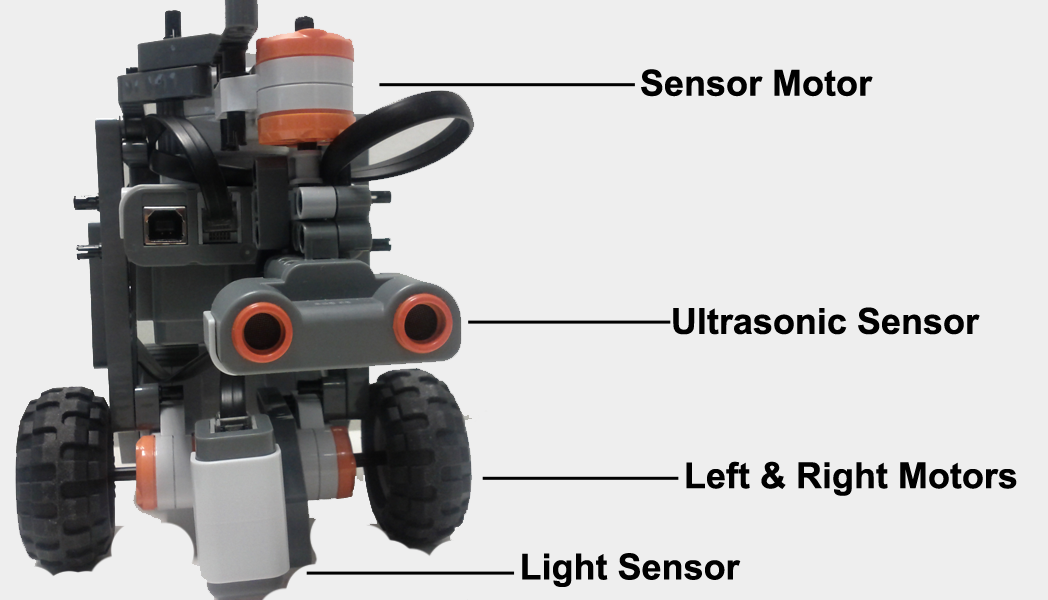
\includegraphics[scale=0.388]{./image/robot1.png}
\end{center}
\vskip 20pt
\begin{center}
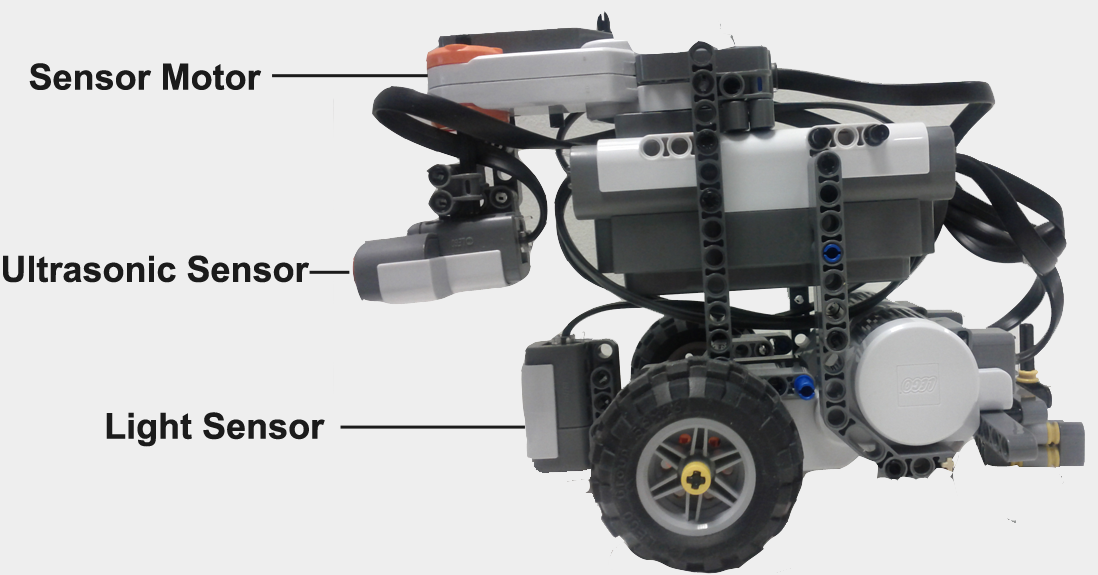
\includegraphics[scale=0.37]{./image/robot2.png}
\end{center}

\begin{center}
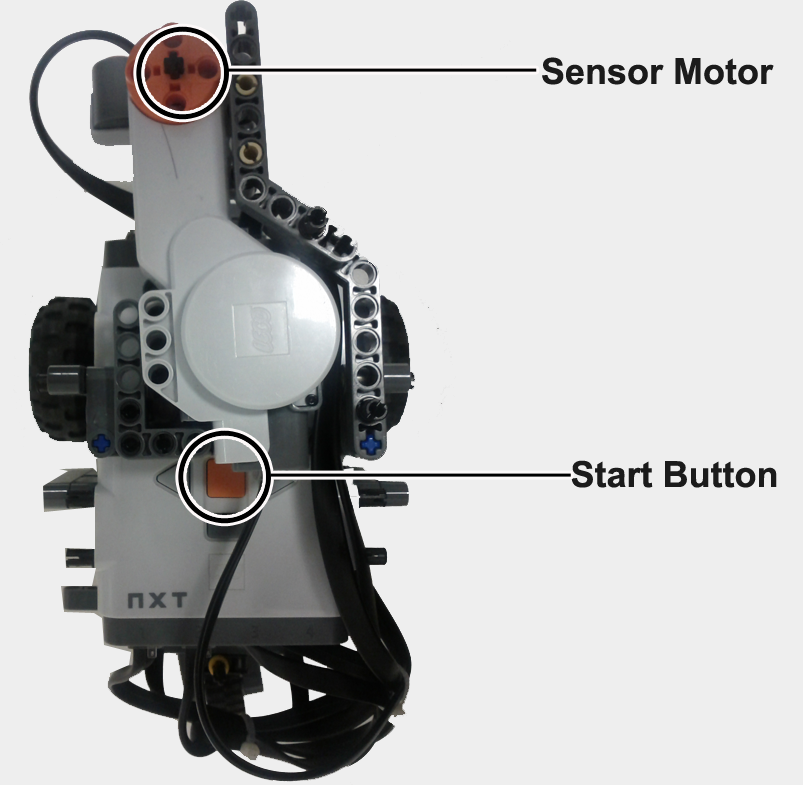
\includegraphics[scale=0.4]{./image/robot3.png}
\end{center}

The NXT Archeology robot consist of LEGO units. There are several parts that are important to the robot. 

\section{Ultra Sonic sensor}
The ultrasonic sensor is installed at the front of the robot. It is used to detect the obstacle at the front, left and right. It can also locate the wall by ultrasonic, thus when robot find a wall, it will be displayed on the map at the corresponding position. Please note that ultrasonic sensor only finds walls location at manual scan mode and automatic mode. However, in manual control mode, ultrasonic sensor is also turned on. When you are moving towards a wall in manual control mode, robot will stop in a distance before it hits the wall, and you will not be able to move any closer to the wall. This is for preventing from damaging the robot.


\section{Sensor Motor}
Sensor Motor is the motor to turn the ultrasonic sensor left, right or front. To accurately map the walls ultra sensor motor will only turn the sensor to three directions. Please make sure the ultrasonic sensor is facing the front before you start. Because the sensor motor will consider the angle that you started with as front and move accordingly. For example, if the ultrasonic sensor is facing left when you start, sensor motor will not be able to turn left anymore.


\section{Left \& Right Motors}
There are two motors control the robot movement. They are installed at the bottom and connect with wheels. These two wheels are responsible for all the movement of robot including moving forward, moving backward, turn right and turn left. The distance between two wheels is a important parameter of the robot pilot system. Changing the distance may have a effect on accuracy.So please DO NOT change the distance between two wheels by your self. 


\section{Light sensor}
Light sensor which is installed below the ultrasonic sensor is used to discover the hidden wall. On the archeology map, hidden walls are distinct from other area
 in color. Light sensor can tell that which area has different color (usually darker). by that, it can find under-ground walls. Light sensor only turned on in manual scan mode and automatic mode. It can not work on manual control mode. 

% chapter robot_main_components (end)



\chapter{GUI Layout} % (fold)
\label{cha:gui_layout}

\section{Basic Layout} % (fold)
\label{sec:basic_layout}
\begin{center}
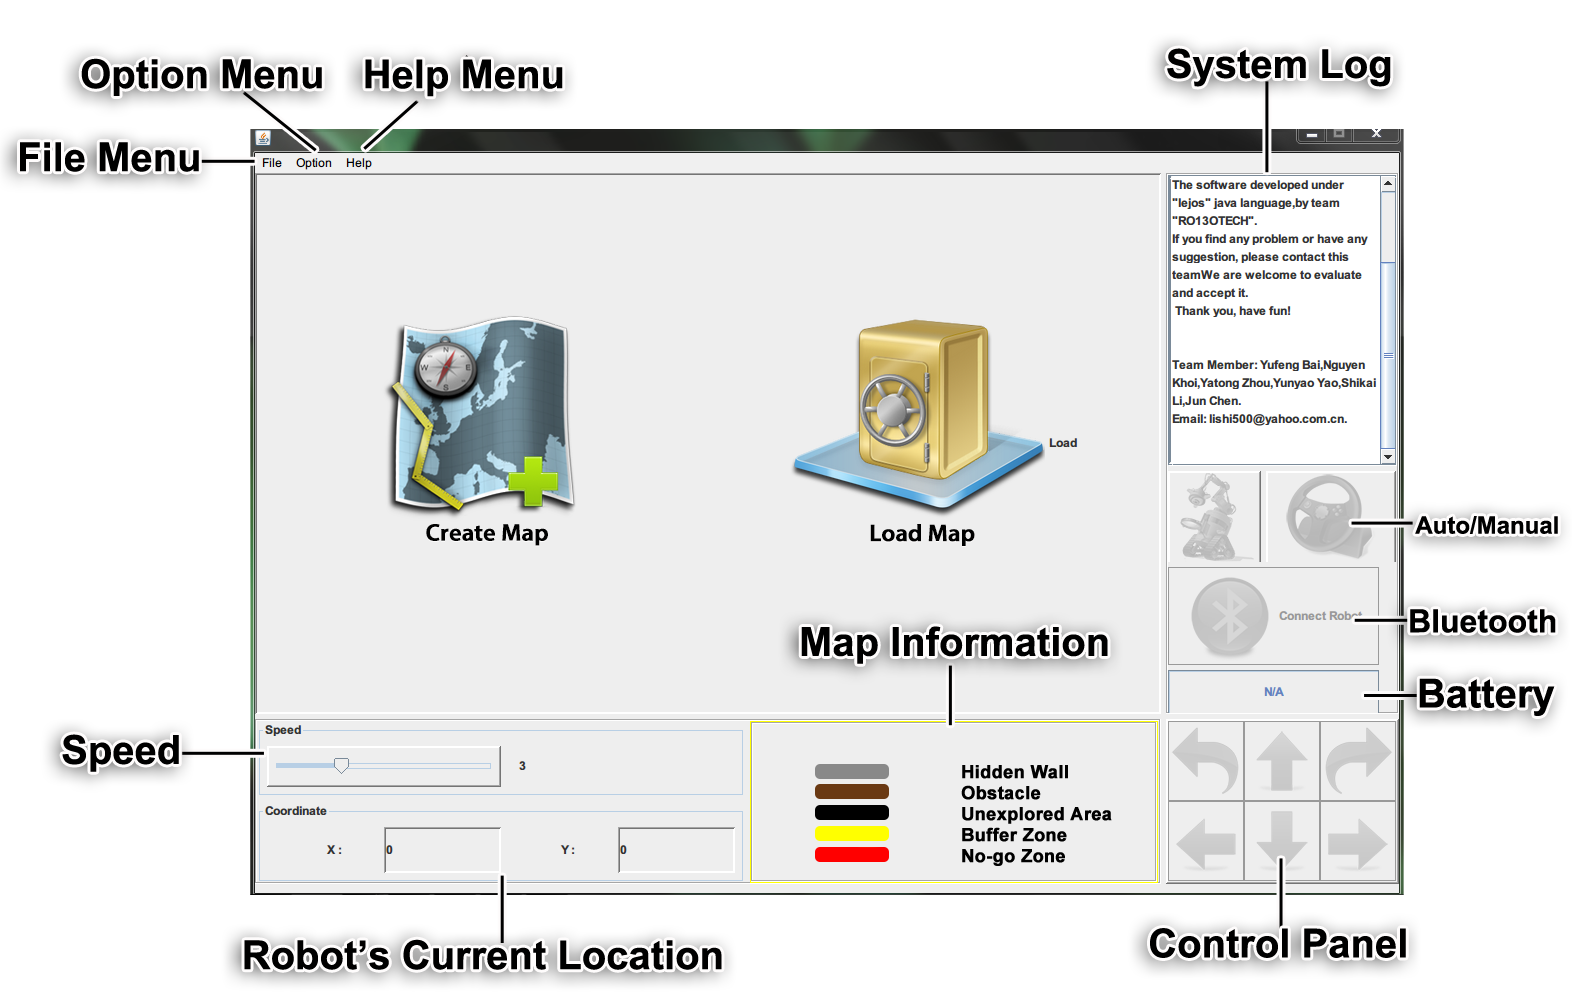
\includegraphics[scale=0.388]{./image/GUIOverview.png}
\end{center}

\begin{itemize}
	\item File menu contains basic XML read \& load operation
	\item Option menu contains the options of auto \& manual navigation, bluetooth control
	\item Help menu contains the version information of this program
	\item System log shows all the log information during the program running
	\item Auto/Manual mode bar can changes the mode of the robot
	\item The bluetooth icon can let the GUI connect the robot
	\item Battery bar shows the battery condition of the robot
	\item Control panel contains the buttons to control the robot manually
	\item Map information shows the colours indicate different type of area
	\item Robot's current location shows the coordinate information of robot
	\item Speed bar can slide and controls the velocity of robot
\end{itemize}



% section basic_layout (end)

\section{Map Panel} % (fold)
\label{sec:map_panel}

\begin{center}
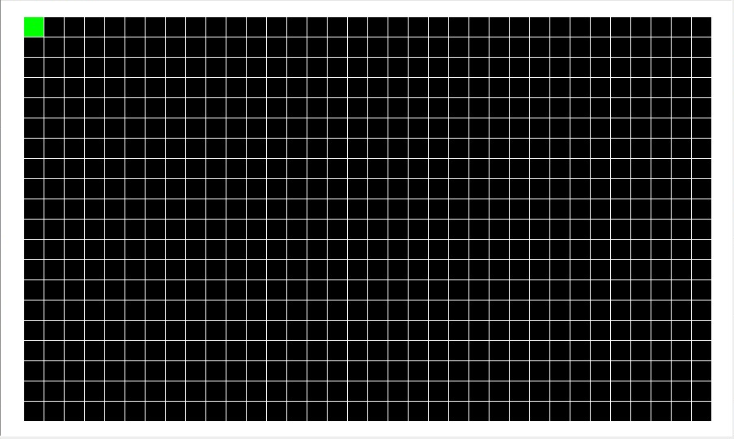
\includegraphics[scale=0.388]{./image/MapArea.png}
\end{center}

\begin{itemize}
	\item Map panel is the main part in the GUI, it displays the map and it will be shown after user create or load a map.\\

	Map panel displays map as pixels. All of the pixels are black initially, which means the map is unexplored, pixel will be refreshed as the robot is scanning. Hidden wall will be gray, and obstacles will be brown. User can bet no go zone, and this terrain will be red. Both no go zone and obstacles will be surrounded a buffer zone, which will be coloured yellow.\\

	Main map panel on the GUI can be dragged with the mouse. It can also be zoomed in/out with the mouse wheel.\\ 
	
\end{itemize}

\begin{center}
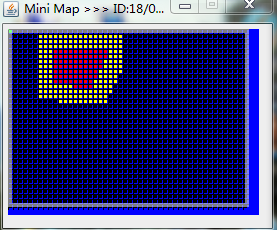
\includegraphics[scale=0.388]{./image/Mini.png}
\end{center}

\begin{itemize}
	\item As the map panel can be zoomed in and only display a part of the map, A mini map will display the whole map in the top left corner. \\
\end{itemize}
% section map_panel (end)


% chapter gui_layout (end)



\chapter{Operation Modes} % (fold)
\label{cha:operation_modes}
Host can operate the robot by three ways: Manual Control, Manual-scan, and Auto-scan.


\section{Manual Control Mode}
When the robot is connected, and user press the Manual Control Mode button in the GUI, the robot enters the Manual Control. User can move robot manually with pressing the ``Up, Down, Left, Right'' buttons to anywhere on the map. However, the map will not be scanned in this mode, that is, any information on the map will not be transferred and displayed on the GUI.
%%%%%%%%picture

\section{Manual-scan Mode}
User can start the robot to Manual-scan Mode when the robot is not operating under auto-scan, in this mode, the robot can scan the map manually after press the ``Option''-``Start Manual-scan'' on the menu bar. In this mode, the robot can be controlled by the user, each movement of the robot will let the robot scan the current pixel information, transfer to the host and display on the map panel of GUI
%%%%%%picture

\section{Auto-scan Mode}
User can set the robot to Auto Mode when the robot is connected, in this mode, the robot can scan the map automatically after press the Option-Start Navigation on the menu bar.
%%%%%%%picture
% chapter operation_modes (end)

\chapter{Getting Started} % (fold)
\label{cha:getting_started}

\section{How to Install} % (fold)
\label{sec:how_to_install}


\subsection{Upload Robot Server} % (fold)
\label{sub:upload_robot_server}
Before upload the robot server, you need to pair with the robot with your computer, if you do not have Bluetooth in your computer, you can use the Bluetooth USB Dongle we provide.\\

Simply add the robot as a device and put the correct pin number (the default pin is ``1234''). If you have any problem pair or connect to the robot, see the chapter \ref{cha:troubleshooting} to find possible solutions.\\

To upload the robot server. Open a command prompt and execute the following command in the directory in which you can see the ``Makefile'':\\
\begin{lstlisting}[language={[ANSI]C}, keywordstyle=\color{blue!70}, commentstyle=\color{red!50!green!50!blue!50}, frame=shadowbox, rulesepcolor=\color{red!20!green!20!blue!20}]
make upload
\end{lstlisting}

After robot server is uploaded, you can continue to compile, install, and run the host program.\\
% subsection upload_robot_server (end)

\section{Compile \& Run the Program} % (fold)
\label{sec:compile_&_run_the_program}

To compile and run the host program for the very first time, you can execute the following command in the same directory before:\\
\begin{lstlisting}[language={[ANSI]C}, keywordstyle=\color{blue!70}, commentstyle=\color{red!50!green!50!blue!50}, frame=shadowbox, rulesepcolor=\color{red!20!green!20!blue!20}]
make run
\end{lstlisting}

After the very first compile, you can execute the host program by:
\begin{lstlisting}[language={[ANSI]C}, keywordstyle=\color{blue!70}, commentstyle=\color{red!50!green!50!blue!50}, frame=shadowbox, rulesepcolor=\color{red!20!green!20!blue!20}]
make exe
\end{lstlisting}

If the program compiled successfully, you can now see the GUI of the program shows up on your screen.\\
\pagebreak


% section compile_&_run_the_program (end)
% section how_to_install (end)


\section{Start Operation} % (fold)
\label{sec:start_operation}
Here is a set of steps to start and complete a operation:

\begin{enumerate}
	\item {Preparation: }Before anything started, you should check if the robot's battery if fully charged, robot's parts if not missing(check the Appendix \ref{cha:parts_list} for more information). 
	\item {Start Robot Server: }Push the ``start button'' on the robot to start the robot server.
	\item {Run the Host Program: }Use the ``Makefile'' to compile and run the host program for the first time or double click the ``RO13TECH.jar'' once you done compile it.
	\item {Create a New Map or Load a XML file: }If you want to create a new map, you may asked to input all the information about the map and the start point for the robot for the robot. If you load a previous map which stored as a XML file, you may start where you left off.
														\begin{figure}[ht]
														\centering
														\setlength\fboxsep{2pt}
														\setlength\fboxrule{0.2pt}
														\fbox{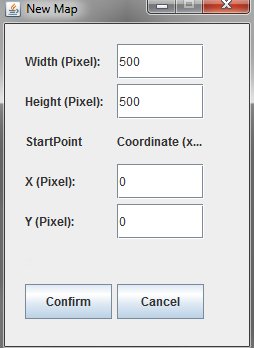
\includegraphics[width =0.3\linewidth]{./image/MapInit.png}}
														\caption{Map Create Panel}
														\label{sec:mcp}
														\label{fig:mcp}
														\end{figure}
														%\pagebreak

	\item {Setting No-go Zones: }You locate a no-go zone by click four points on the map. You can create multiple no-go zones by repeat doing this. You can also ``Undo'' and ``Redo'' your settings.

														\begin{figure}[ht]
														\centering
														\setlength\fboxsep{2pt}
														\setlength\fboxrule{0.2pt}
														\fbox{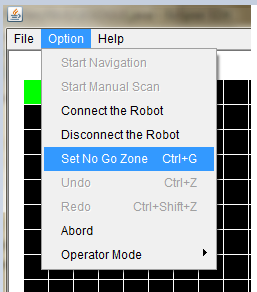
\includegraphics[width =0.3\linewidth]{./image/NoGoZone.png}}
														\caption{Set No-go Zone}
														\label{sec:sn}
														\label{fig:sn}
														\end{figure}
														\pagebreak
	\item {Connect: }Click the Bluetooth icon to start connect to the robot. System log will shows ``Start Control'' once the connection is created.
														\begin{figure}[ht]
														\centering
														\setlength\fboxsep{2pt}
														\setlength\fboxrule{0.2pt}
														\fbox{
\includegraphics[width =0.3\linewidth]{./image/Bluetooth.png}}
														\caption{Activated Bluetooth Icon}
														\label{sec:bi}
														\label{fig:bi}
														\end{figure}
														%\pagebreak
	\item {Start Manual Control to Get to Start Point: }Click the Manual Control icon to start manual control, control the robot using the Control Panel. Control the robot reach the start point which you setted on the map.
	\item {Start Auto-scan or Manual-scanL: }Make sure the robot is at the start point, you can start Auto-scan or Manual-scan. 
														\begin{figure}[ht]
														\centering
														\setlength\fboxsep{2pt}
														\setlength\fboxrule{0.2pt}
														\fbox{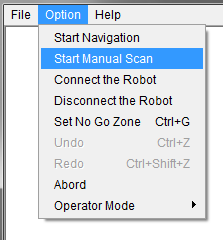
\includegraphics[width =0.3\linewidth]{./image/ManScan.png}}
														\caption{Scan Options}
														\label{sec:so}
														\label{fig:so}
														\end{figure}
														%\pagebreak

	\item {Stop operation: }If you wish to stop the operation, simply click ``Stop Operation'', robot will be stopped and waiting for further instructions.
	\item {Operation Complete: }After the map is fully scanned, robot will return to the start point. If you choose to stop the operation, then you may manually control the robot go back to the start point.\pagebreak
	\item {Save the Map: }Finally, you can save the map to a XML file to finish up the operation.
														\begin{figure}[ht]
														\centering
														\setlength\fboxsep{2pt}
														\setlength\fboxrule{0.2pt}
														\fbox{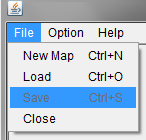
\includegraphics[width =0.3\linewidth]{./image/SaveMap.png}}
														\caption{Save the Map}
														\label{sec:sm}
														\label{fig:sm}
														\end{figure}
														%\pagebreak

\end{enumerate}

% section start_operation (end)



% chapter getting_started (end)






\chapter{Features for Power User} % (fold)
\label{cha:features_for_power_user}

\section{Maintenance Mode} % (fold)
\label{sec:maintance_mode}
In maintenance mode user are allowed to set the Robot's speed and override system variables. Such feature requires experience with the robot and the system, so do not try to switch to the maintenance mode at first-time use.\\
Robot is running at speed level three as default, however, before or during the manual control, you can switch to maintenance mode and set the robot's speed from one to ten as you want.\\
More features will be updated in further release.\\

\section{Keyboard Short-cut} % (fold)
\label{sec:keyboard_short_cut}
Keyboard short-cut is provided for the user, you can use:
\begin{enumerate}
 	\item ``Ctrl-N'' to create new map.
 	\item ``Ctrl-O'' to load XML file.
 	\item ``Ctrl-S'' to save current map.
 	\item ``Ctrl-G'' to set no-go zone.
 	\item ``Ctrl-Z'' to Undo your setted no-go zone.
 	\item ``Shift-Ctrl-Z'' to Redo your setted no-go zone.
 \end{enumerate}
  
% section keyboard_short_cut (end)



% section maintance_mode (end)




\chapter{Maintenance of the Hardware} % (fold)
\label{cha:maintenance_of_the_hardware}

\section{Battery Maintenance} % (fold)
\label{sec:battery_maintenance}

% section battery_maintenance (end)
The battery of the robot displays on the Appendix A Part List No.6.\\
If the user want to buy the new battery, the website shows below:\\
\url{http://education.lego.com/en-us/lego-education-product-database/mindstorms/9693-rechargeable-battery-dc/}\\ 
The Battery Maintenance is an important issue. Extreme heat and cold, alternator undercharging or overcharging all reduce the life time of the battery. The battery should be cleaned using a baking soda and water solution; a couple of table spoons to a pint of water. Cable connections need to be cleaned and tightened as battery problems are often caused by dirty and loose connections. \\ 
For the safety of the battery, the user is highly suggested to follow the suggestion below:
\subsection{Battery Do's}
\begin{enumerate}
\item Read entire tutorial carefully.
\item Do regular inspection and maintenance especially in hot weather.
\item Do recharge battery immediately after using it. 
\item if the battery level is lower than 20 percent, the user need to charge immediately.
\item When the user does not use the battery, please keep the battery in the dry and shady environment.
\end{enumerate}
\subsection{Battery Don'ts}
\begin{enumerate}
\item Do not expose the battery on the hard light environment.
\item Do not put the battery on the moist environment.
\item Do not use unregulated high output battery chargers to charge batteries.
\item Do not let a battery get hot to the touch and boil violently when charging.
\item Do not charging the battery more than 10 hours one time.
\item Do not mix size and types of batteries.
\item Do not squeeze the battery.
\end{enumerate}
\section{Robot Hardware Maintenance} % (fold)
\label{sec:robot_hardware_maintenance}
The hardware includes all components, which are used to build the robot. The hardware has a significant influence on the operation and accuracy of the robot. It is necessary to keep the every part of the robot complete. if the user want to buy the relevant component of the robot, the website shows below:\\ 
\url{http://search2.lego.com/?q=mindstorm&lang=2057&cc=US} \\ 
For the safety of the battery, the user is highly suggested to follow the suggestion below:
\subsection{Hardware Do's}
\begin{enumerate}
\item Keep cleaning every component of the robot frequently.
\item After using the robot, make sure every part is kept in the robot box.
\item Test the sensors frequently to make sure they work correctly.
\end{enumerate}
\subsection{Hardware Don'ts}
\begin{enumerate}
\item Do not expose the hardware on the hard light environment.
\item Do not put the hardware on the moist environment.
\item Do not squeeze the hardware.
\end{enumerate}
% section robot_hardware_maintenance (end)



% chapter maintenance_of_the_hardware (end)








% chapter features_for_power_user (end)


\chapter{Troubleshooting} % (fold)
\label{cha:troubleshooting}
\begin{enumerate}
	\item  For the user who is running Mac OS X Mountain Lion, you may having some issues connecting the robot. You can solve this problem by installing a lower version of OS X(ie: OS X Lion 10.7.X) or according to \href{https://groups.google.com/forum/?fromgroups=#!topic/bluecove-users/7jWv1V1GC-4}{this}, try to use the \href{https://bluecove-users.googlegroups.com/attach/8c4cbcadb7aa9e5/IOBluetooth-Lion.tgz?pli=1&view=1&part=4}{blue-tooth framework} of OS X Lion. 

	\item Users who using both 32 bit and 64 bit JRE and JDK may have problem run the program after you compile it. That is because the LejOS library does not support 64 bit JRE and JDK, using the JVM argument ``-d32'' to solve this problem.

	\item Some situations may freeze the robot's server program which you can not reboot the robot by close the host program. Simply remove the robot's battery and put it back in to solve this problem.

\end{enumerate}

We are happy to receive your problems and suggestions, sending us a \href{ro13botech@gmail.com}{email} to get any question answered and out latest updates.
% chapter troubleshooting (end)





\newpage
\appendix

\chapter{Parts List} % (fold)
\label{cha:parts_list}

\begin{enumerate}
	\item  Lego Mindstorms 9847 Bluetooth® Dongle * 1. 
		\begin{figure}[ht]
		\centering
		\setlength\fboxsep{2pt}
		\setlength\fboxrule{0.2pt}
		\fbox{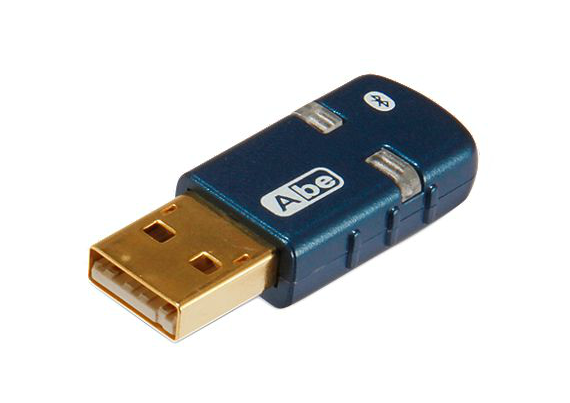
\includegraphics[width =0.3\linewidth]{./image/bluetoothDongle.png}}
		\caption{Lego Mindstorms 9847 Bluetooth® Dongle}
		\label{sec:bd}
		\label{fig:bd}
		\end{figure}
	\item  Lego Mindstorms 9844 Light Sensor * 1.\begin{figure}[ht]
		\centering
		\setlength\fboxsep{2pt}
		\setlength\fboxrule{0.2pt}
		\fbox{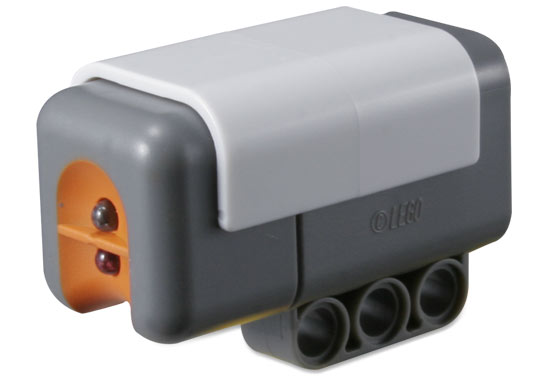
\includegraphics[width =0.3\linewidth]{./image/Light.jpg}}
		\caption{Lego Mindstorms 9844 Light Sensor}
		\label{sec:ls}
		\label{fig:ls}
		\end{figure}
		%\pagebreak
	\item  Lego Mindstorms 9846 Ultrasonic Sensor * 1.
		\begin{figure}[ht]
		\centering
		\setlength\fboxsep{2pt}
		\setlength\fboxrule{0.2pt}
		\fbox{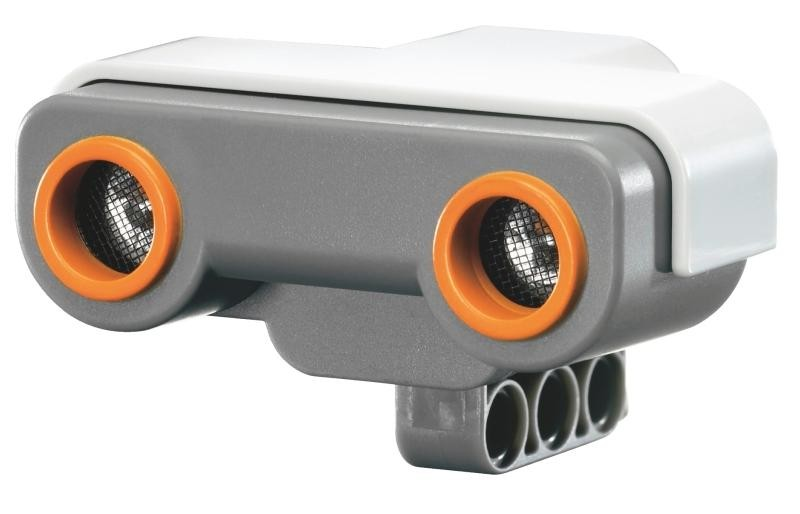
\includegraphics[width =0.3\linewidth]{./image/Ultrasonic.jpg}}
		\caption{Lego Mindstorms 9846 Ultrasonic Sensor}
		\label{sec:us}
		\label{fig:us}
		\end{figure}
		\pagebreak
	\item  Lego Mindstorms 9842 Interactiv Servo Motor * 3.
		\begin{figure}[ht]
		\centering
		\setlength\fboxsep{2pt}
		\setlength\fboxrule{0.2pt}
		\fbox{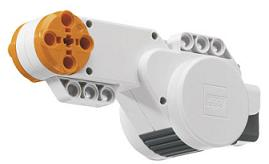
\includegraphics[width =0.3\linewidth]{./image/Motor.jpg}}
		\caption{Lego Mindstorms 9842 Interactiv Servo Motor}
		\label{sec:ism}
		\label{fig:ism}
		\end{figure}
	\item  Lego Mindstorms 9841 NXT Intelligent Brick * 1.
		\begin{figure}[ht]
		\centering
		\setlength\fboxsep{2pt}
		\setlength\fboxrule{0.2pt}
		\fbox{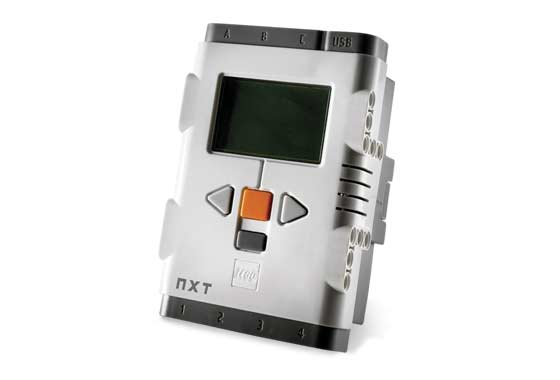
\includegraphics[width =0.3\linewidth]{./image/Brick.jpg}}
		\caption{Lego Mindstorms 9841 NXT Intelligent Brick}
		\label{sec:ib}
		\label{fig:ib}
		\end{figure}
	\item  Lego Mindstorms 9693 Rechargeable Battery * 1
		\begin{figure}[ht]
		\centering
		\setlength\fboxsep{2pt}
		\setlength\fboxrule{0.2pt}
		\fbox{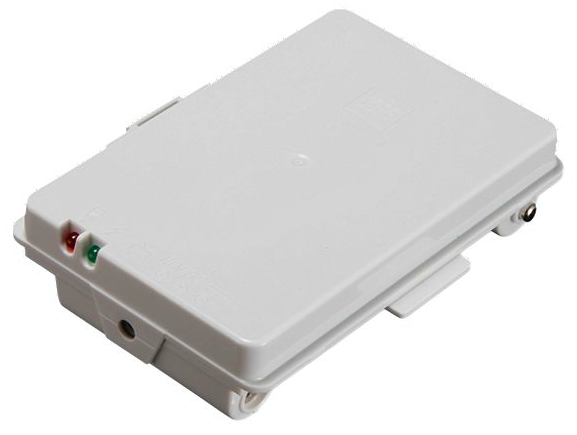
\includegraphics[width =0.3\linewidth]{./image/Battery.png}}
		\caption{Lego Mindstorms 9693 Rechargeable Battery}
		\label{sec:battery}
		\label{fig:battery}
		\end{figure}
\end{enumerate}

% chapter parts_list (end)




\chapter{Glossary}


\paragraph{GUI:} Acronym of Graphic User Interface. This is what is used to display map and control panel

\paragraph{Control Panel:} The manual control panel.

\paragraph{No-Go Zone:} A zone which the robot is forbidden to enter.

\paragraph{Pixel:} The smallest addressable element in a display device.

\paragraph{Square:} The smallest addressable element in the map.

\paragraph{Lejos:} A firmware replacement for Lego Mindstorms programmable bricks, which allows Lego Mindstorms robots to be programmed in the Java programming language.


\pagebreak{}






\end{document}

